\documentclass[executivepaper]{article}

\usepackage{mathtools}

\everymath{\displaystyle}

\usepackage{amssymb}

\usepackage{kantlipsum,graphicx}

\usepackage{amsmath}

\usepackage[utf8]{inputenc}

\usepackage{sectsty}

\sectionfont{\large}

\subsectionfont{\normalsize}

\begin{document}

\vspace*{-40mm}

\section*{Experimental Results}

Below are some of the experimental results that lead to the observation that is presented in the next section

\begin{center}

\begin{tabular}{||c c c c||}

\hline

$\lambda$ & $M$ & $N$ & Roots \\ [0.5ex]

\hline\hline

4 & 0 & 2 & 0.2, Asymptotic Behaviour down at 0.2 \\ 

\hline

7 & 0 & 2 & 0.3, 0.1, Asymptotic Behaviour up at 0.1 \\

\hline

15 & 0 & 2 & 0.45, 0.2, 0.1, Asymptotic Behaviour down at 0.1 \\

\hline

17 & 0 & 2 & 0.47, 0.22, 0.1, Asymptotic behaviour up at 0.05 \\
\hline

22 & 0 & 2 & 0.5, 0.27, 0.12, 0.05, Asymptotic behaviour at 0.03 \\ [1ex]

\hline

\end{tabular}

\begin{figure}[!ht]

\centering

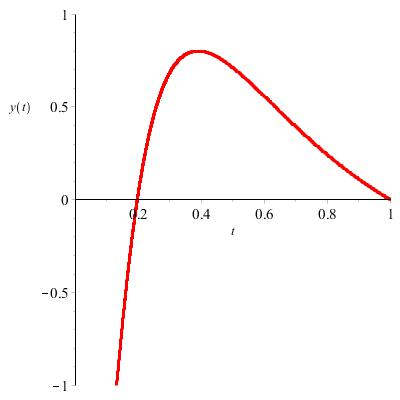
\includegraphics[width=0.5\textwidth]{NEquals2MEquals0LambdaEquals4}

\caption{$N=2$, $M=0$, and $\lambda=4$}

\end{figure}

\vspace{5mm}

\begin{figure}[!ht]

\centering

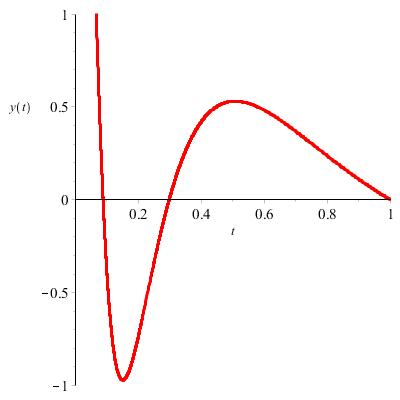
\includegraphics[width=0.5\textwidth]{NEquals2MEquals0LambdaEquals7}

\caption{$N=2$, $M=0$, and $\lambda=7$}

\end{figure}

\vspace{5mm}

\begin{figure}[!ht]

\centering

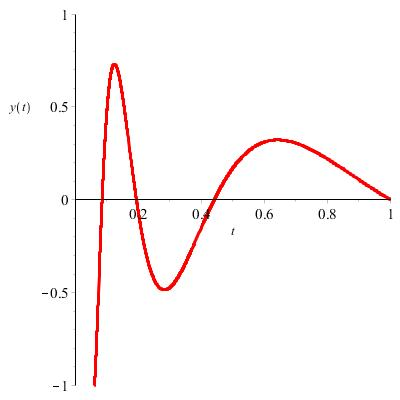
\includegraphics[width=0.5\textwidth]{NEquals2MEquals0LambdaEquals15}

\caption{$N=2$, $M=0$, and $\lambda=15$}

\end{figure}

\vspace{5mm}

\begin{figure}[!ht]

\centering

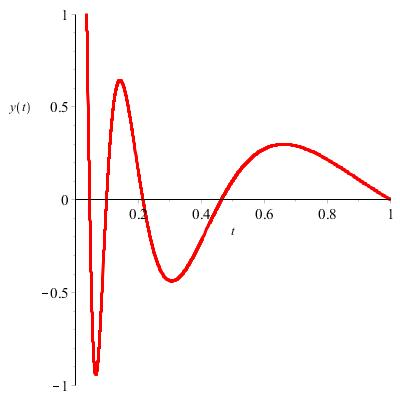
\includegraphics[width=0.5\textwidth]{NEquals2MEquals0LambdaEquals17}

\caption{$N=2$, $M=0$, and $\lambda=17$}

\end{figure}

\vspace{5mm}

\begin{figure}[!ht]

\centering

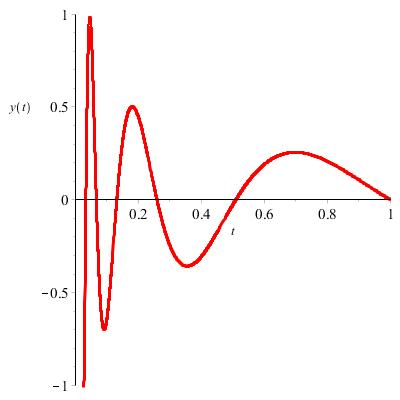
\includegraphics[width=0.5\textwidth]{NEquals2MEquals0LambdaEquals22}

\caption{$N=2$, $M=0$, and $\lambda=22$}

\end{figure}

\end{center}

\end{document}